\tikzset{
    curve-technique/.pic = {
        \fill[#1, opacity = 0.3] (-2, 0) arc (180:360:2) to[out = 90, in = 0] (0, 4) to[out = 180, in = 90] (-2, 0) -- cycle;
        \draw[#1!80, thick] (-2, 0) arc (180:360:2) to[out = 90, in = 0] (0, 4) to[out = 180, in = 90] (-2, 0) -- cycle;
    }
}
    

    
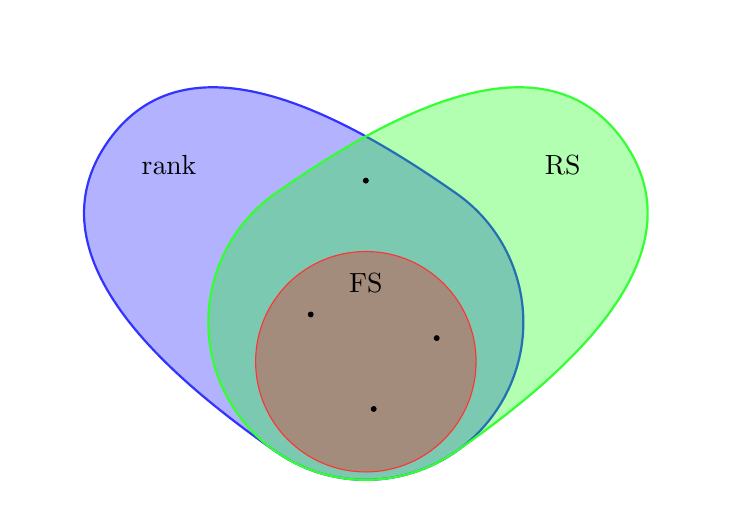
\begin{tikzpicture}[>=latex]
    \pic[rotate = 55] {curve-technique = {blue}};
    \pic[rotate = -55] {curve-technique = {green}};

    \fill[red, opacity = 0.3] (0, -0.5) circle (1.4);
    \draw[red!80] (0, -0.5) circle (1.4);

    \node at (0, 0.5) {FS};
    \node at (-2.5, 2) {rank};
    \node at (2.5, 2) {RS};

    \draw[fill = black] (-0.7, 0.1) circle (0.03) node[below] {$\EQ$};
    \draw[fill = black] (0.9, -0.2) circle (0.03) node[below] {$\GT$};
    \draw[fill = black] (0.1, -1.1) circle (0.03) node[below] {$\Disj$};

    \draw[fill = black] (0, 1.8) circle (0.03) node[below] {$\IP$};
\end{tikzpicture}